 \chapter{Energy Model}
 This chapter presents a simplified energy model based on the measurement and theory section. 
 \subsection{Data analysis}
 The first step in making an energy model of the GPS receiver is to analyze the data from the measurements and relating it to the theory. The theory section explains how the receiver operates between two distinct phases: acquisition and tracking. The two phases can be modelled in a state diagram. 
 
 
\begin{figure}[H]
\centering
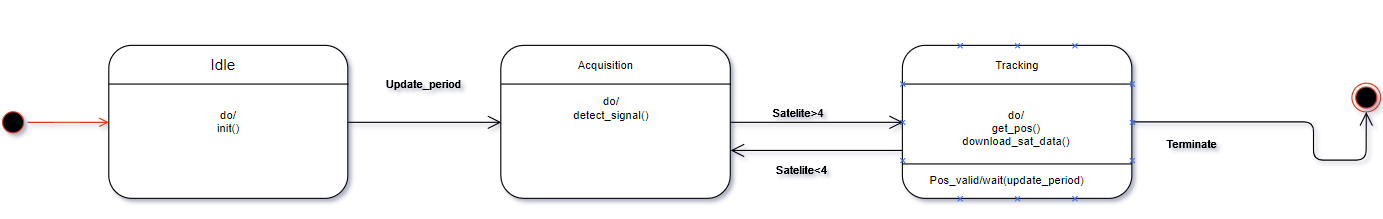
\includegraphics[width=16 cm]{Project_Report/Images/gps_basics.PNG}
\caption{The state diagram of a GPS receiver}
\label{fig:GPS reciever}
\end{figure}
 
 The trigger functionality from \ref{fig:WIFI_OFF} highlights when the receiver has a positional fix. We know from the theory, that the receiver switches to the tracking phase when it acquires a positional fix. This means that the GPS is in the tracking phase, the instant the trigger is set. The trigger functionality can't however, inform about later transitions because the receiver changes phases after it has a positional fix. The receiver does this to maintain its signal strength. The state diagram for the LoPy is an extension of \ref{fig:GPS reciever} with deepsleep and timeout. The extended state diagram is show in figure \ref{fig:GPS energymodel}
 
\begin{figure}[h]
\centering
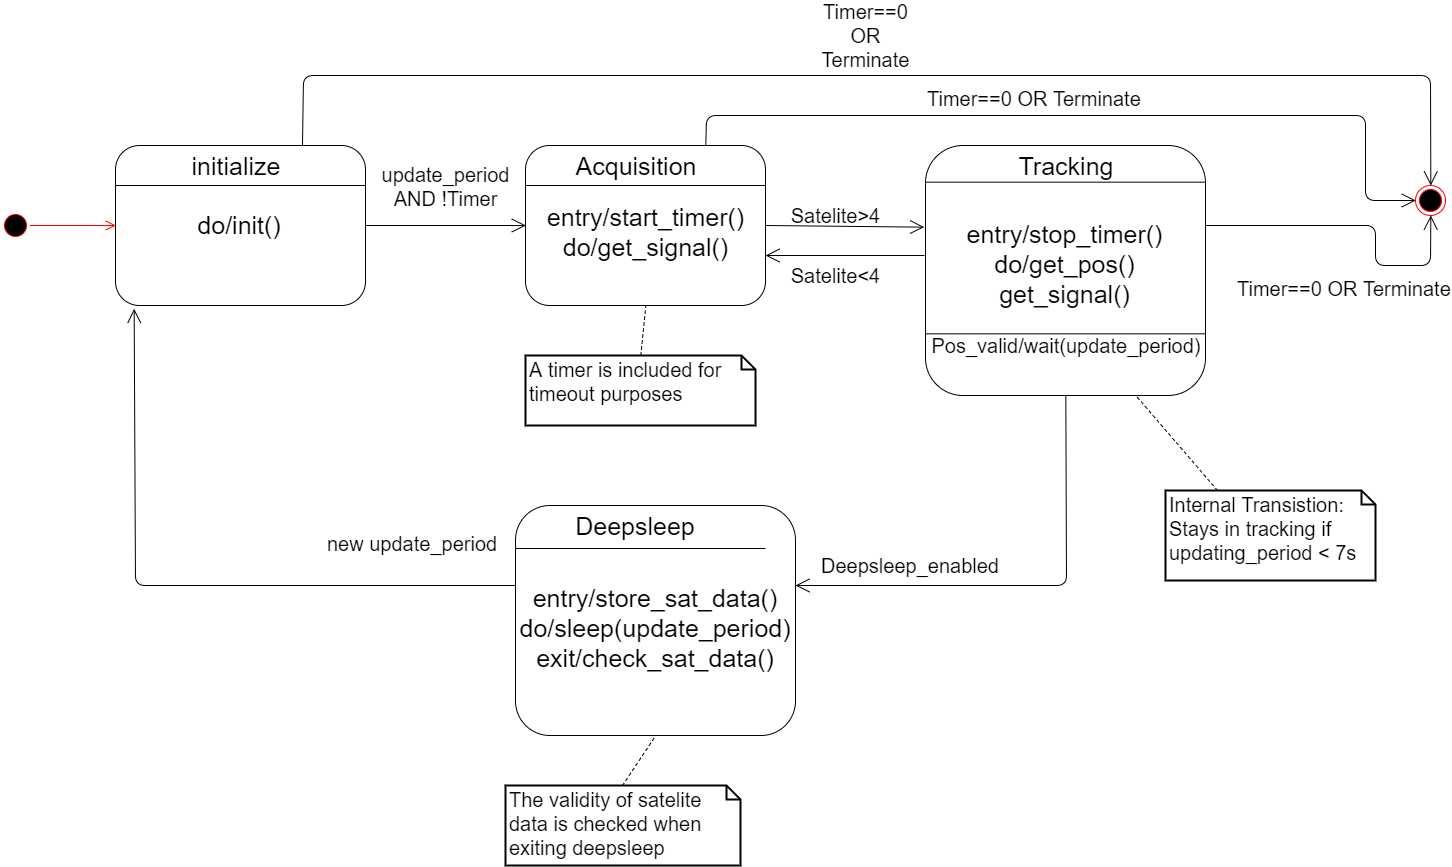
\includegraphics[width=15 cm]{Project_Report/Images/Energymodel.png}
\caption{The state diagram of the LoPy}
\label{fig:GPS energymodel}
\end{figure}
 
A table with the data of the current consumption right before and after the trigger is set, is generated in a acquisition and a tracking column respectively. The average of each column is calculated. A screenshot of the data along with the scatter plots for each column is shown in \ref{fig:average}
 
\begin{figure}[H]
\centering
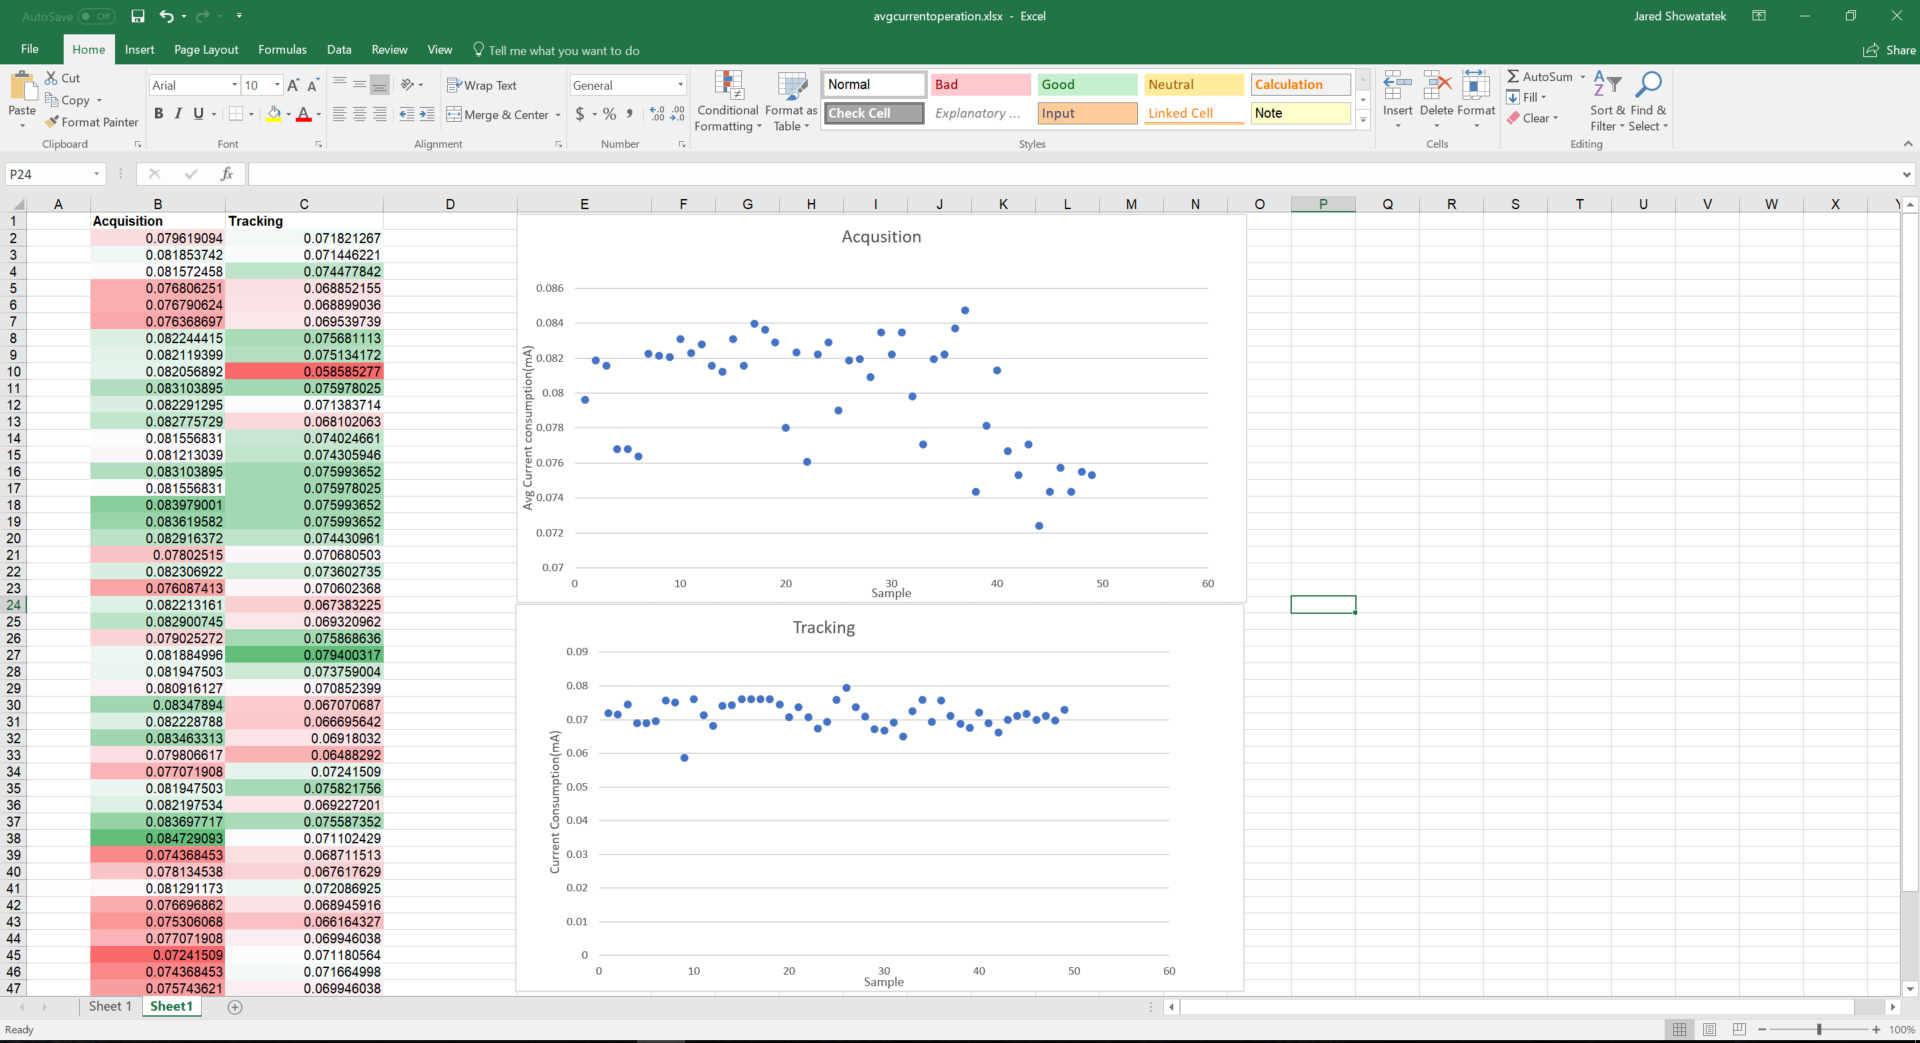
\includegraphics[width=15 cm]{Project_Report/Images/average.PNG}
\caption{The average values for acquisition and tracking phase }
\label{fig:average}
\end{figure}
 
 Average value of the acquisition and tracking phase is calculated to 80 mA and 72 mA respectively. \ref{fig:average} shows how the current consumption is decreasing in both of the states in the later measurements. The schematics from \ref{fig:LoPy_Schematic} shows that the LoPy is using a LiPo battery for voltage supply. Rechargeable batteries  tend to have a discharge curve, which means that the battery voltage changes during discharge. This affect might be the cause of the deviating voltage values in the later measurements. 
 
 The average values are compared with the features from the datasheet \cite{L76}. The datasheet state, that it should be a 7 mA difference between the acquisition and tracking phase. This seems to validate the measurements, which shows a decreasing in current consumption from 80 mA to 71 mA after a positional fix.   
 
 
\subsection{The model}
 
 
The python script in appendix \ref{Appendix:make_energy_model.py} use a simplified energy model to calculate the energy consumption over a fix period.
A fix period is defined as the duration the microcontroller use to acquire a fix from deepsleep:

\begin{equation}
E_{fixperiod} = P_{fixperiod}*T_{fixperiod}
\end{equation}
During a fix period, the microcontroller transitions between the states in figure \ref{fig:GPS energymodel}. The total energy consumption $E_{fixperiod}$ can then be written as the sum of the energy of each state:

\begin{equation}
E_{fixperiod} = P_{Idle}*T_{Idle} + P_{Acquisition}*T_{Acquisition} + P_{Tracking}*T_{Tracking} + P_{Deepsleep}*T_{Deepsleep}
\end{equation}
\begin{equation}
T_{Deepsleep} = {T_fixperiod} - {T_idle} - {T_Acquisition} - {T_Tracking}
\end{equation}
$T_ {Acquisition}$ depends on the last fix which is given by the $fix_period$.
The total energy consumption over a duration t is given by the energy consumption of a fix period multiplied by the number of periods during the total duration t.

\begin{equation}
 E_{total} = E_{fixperiod}* \frac{t}{fixperiod}
\end{equation}

Table \ref{Table:data for the energy model} shows the data that is used in the python script. The power is plotted in a pie diagram in figure \ref{fig:powerconsumption}
\begin{table}[h!]
\begin{center}
 \begin{tabular}{||c c c||} 
 \hline
  State & Time(s) & Power(W) \\ [0.5ex] 
 \hline\hline
  Idle & 5 & 10.201 \\ 
 \hline
 Acquisition & 1/30/35 & 6.4 \\
 \hline
 Tracking & 1 & 5.0 \\
 \hline
 Deepsleep &  & 0.01 \\
 [1ex]
 \hline
\end{tabular}
\end{center}
\caption{Data that is used for the energy model}
\label{Table:data for the energy model}
\end{table}

\begin{figure}[H]
\centering
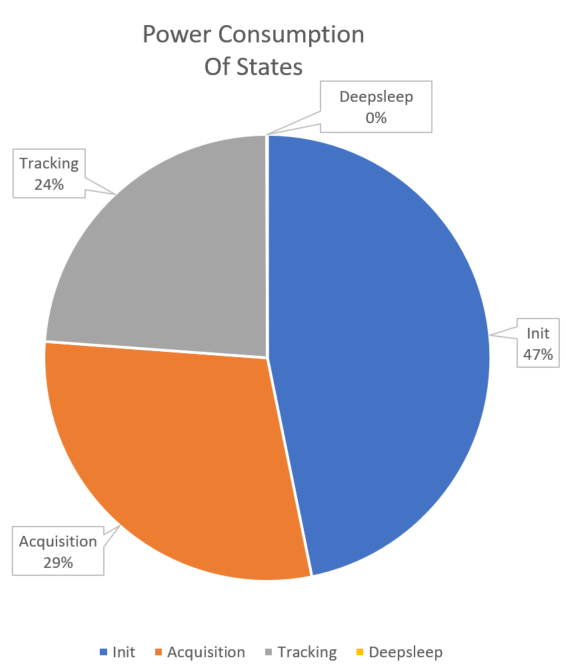
\includegraphics[height=7.5cm]{Project_Report/Images/powerconsump.PNG}
\caption{The pie diagram of the power in table \ref{Table:data for the energy model}}
\label{fig:powerconsumption}
\end{figure}

The values used for time in acquisition, depends on the validity of satellite data. The times that are given in table \ref{Table:data for the energy model} is from the specification \cite{L76}.
The python scripts generates an Excel sheet with the energy consumption for measuring the energy consumption of different fix periods over different durations. The data is given in table \ref{Table:energy}

\begin{table}[h!]
\begin{center}
 \begin{tabular}{||c c c c c c||} 
 \hline
 & Duration & & & & \\
 \hline
  & 60s & 1 Hour & 1 day & 30 days & 1 year \\
  Update Period & & & & &  \\[0.5ex] 
 \hline\hline
  1s & 0.3108 & 18.648 & 447.552 & 13426.6 & 163356 \\ 
 \hline
  10s & 0.278236 & 16.69414 & 400.6594 & 12019.78 & 146240.7 \\
 \hline
  60s & 0.046573 & 2.794357 & 67.06456 & 2011.937 & 24478.56 \\
 \hline
  1800s & -1 & 0.107065 & 2.569565 & 77.08696 & 937.8913 \\
  \hline
  3600s & -1 & 0.060733 & 1.457583 & 43.72748 & 532.0177 \\
  \hline
  14399s & -1 & -1 & 0.623615 & 18.70845 & 227.6195 \\
  \hline
  14400s & -1 & -1 & 1.708834 & 51.26501 & 623.7243\\
  \hline
  15551700s & -1 & -1 & -1 & -1 & 126.6047 \\
  \hline
  15552000s & -1 & -1 & -1 & -1 & 126.668 \\[1ex]
 \hline
\end{tabular}
\end{center}
\caption{Table displaying the energy consumption over different durations and update periods}
\label{Table:energy}
\end{table}

An invalid valid of -1 is given for update periods that are larger then the duration. 14400(4 hours) is the limit for the validity of the ephemeris. Having a update frequency 4 hours makes the validity of  ephemeris invalid, and makes the receiver spend 30 seconds instead of 1 second in the acquisition state. The benefit of having an updating period that is less than 4 hour, instead of just over 4 hours is shown in the table \ref{Table:energy}. The table shows that this strategy will save  $623.72 - 227.61 = 396.11 J$ over a year. A similar analysis is made for the Almanac. 15551700s(179 days) is the limit for the validity of the Almanac. But it isn't a noteworthy reduce of energy over a year:  $126.6047 - 126.668$. This is because of the small time penalty that is associated with an invalid Almanac versus just an invalid  ephemeris. A plot of the energy consumption is shown in figure \ref{fig:energyconsumption}

\begin{figure}[H]
\centering
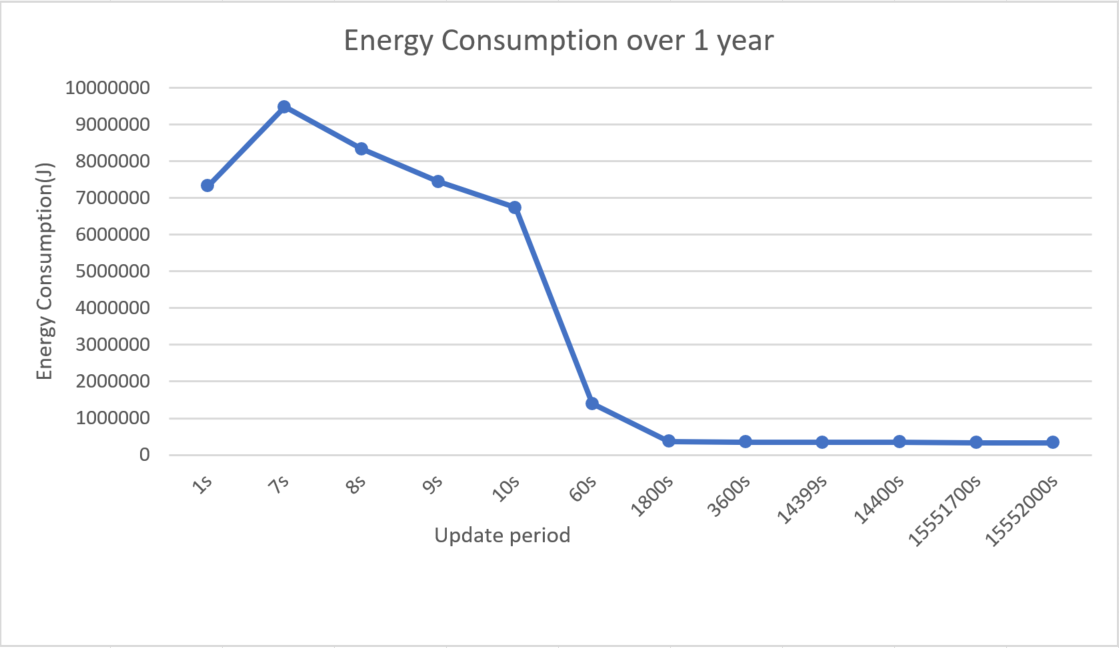
\includegraphics[height=7.0cm]{Project_Report/Images/energyconsumption.PNG}
\caption{The plot of table \ref{Table:energy}}
\label{fig:energyconsumption}
\end{figure}


It is possible to find the limiting updating period for when its more beneficial in terms of energy savings, to have an update frequency under 14400 versus over. The program in \ref{code:limit} uses the data from the energy model to find the limit updating frequency. The result from the execution of the program is shown in \ref{fig:limit}. 



\lstset{language=Python}          % Set your language (you can change the language for each code-block optionally)
\begin{lstlisting}[frame=single, caption= Code used for finding the beneficial limit]  % Start your code-block

    temp    =   Energy_consumption[4][5]
    optimal     =   Energy_consumption[4][6]
    fix_o = 14400

    while(temp<optimal):  
        T_sleep = fix_o - T_wake - 30 - T_track
        optimal = (P_sleep*T_sleep + P_wake*T_wake + P_acq*T_acq + P_track*T_track)*t[4]/fix_o
        print(optimal)
        fix_o = fix_o + 1

    print("Limit updating :",fix_o)
\end{lstlisting}
\label{code:limit}


\begin{figure}[H]
\centering
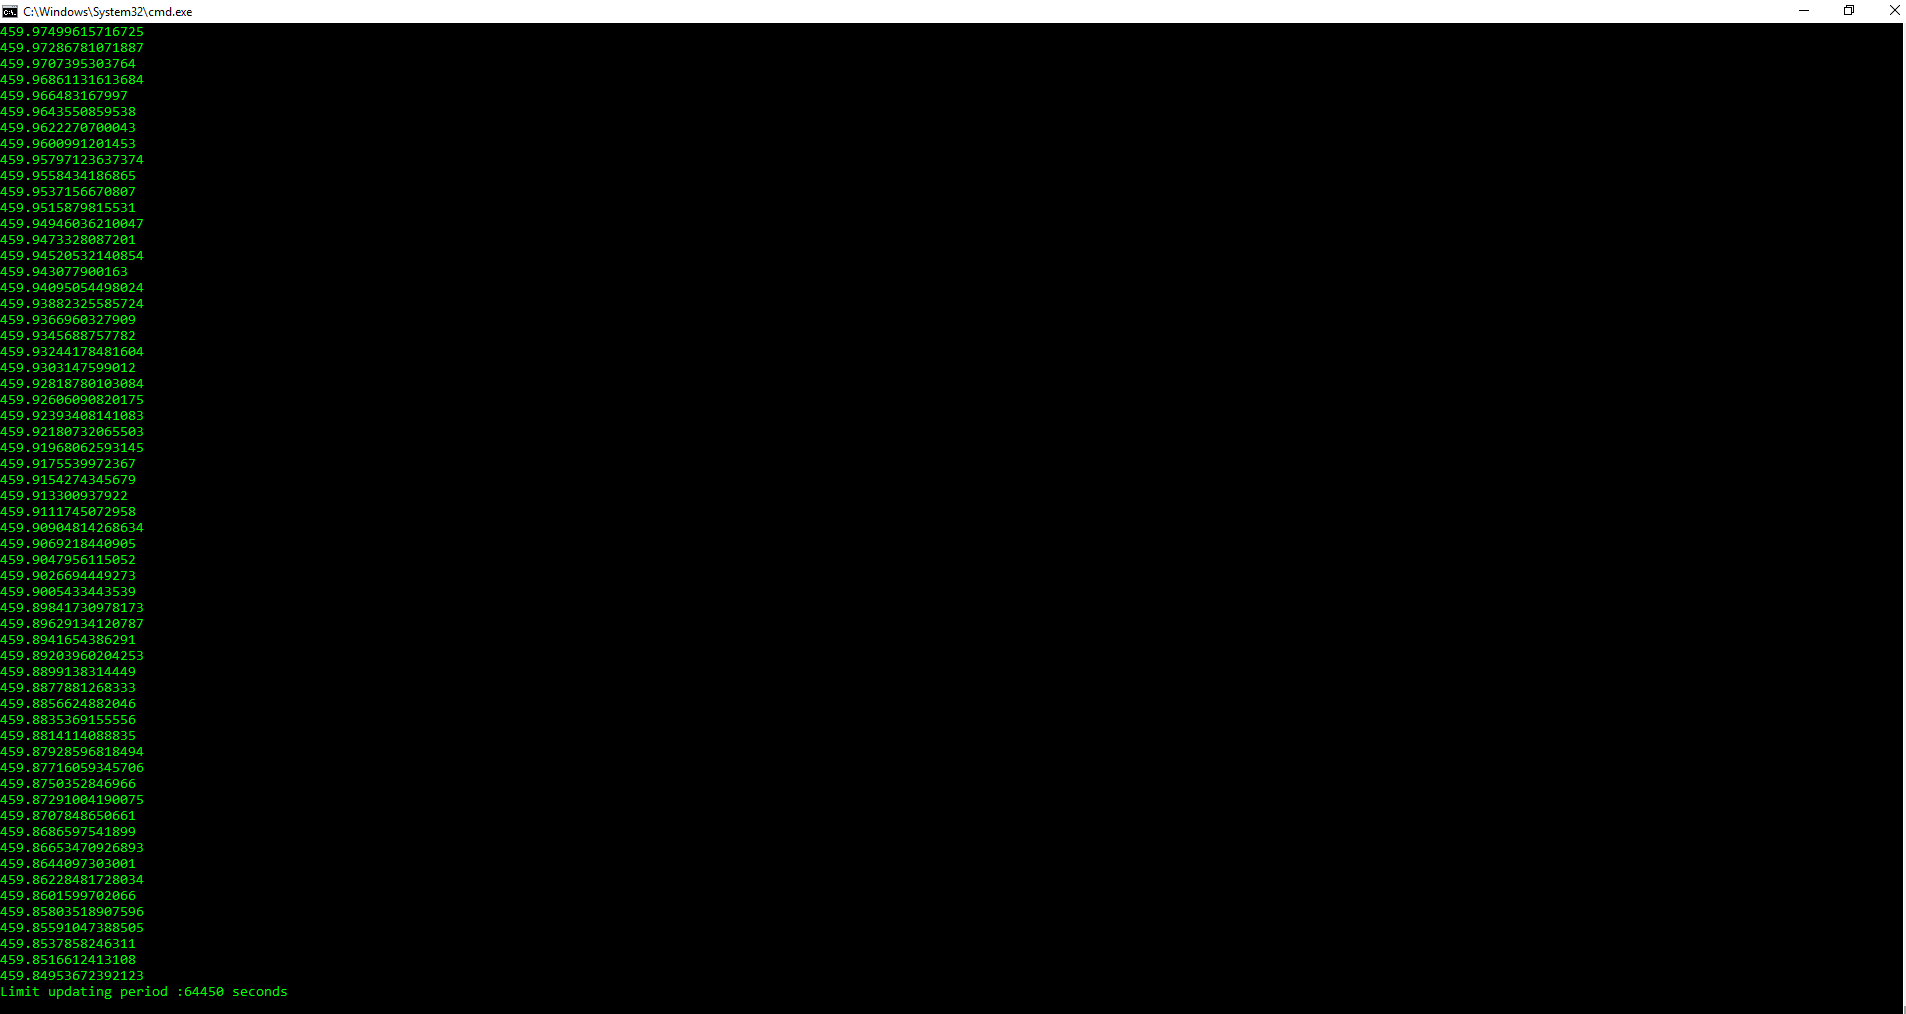
\includegraphics[height=8.0cm]{Project_Report/Images/limit.PNG}
\caption{A screenshot of the execution of the program code in \ref{code:limit}}
\label{fig:limit}
\end{figure}

It is therefore better to have an updating period of just under 4 hours versus having an longer updating period up to 64440 seconds. 



\newpage